% !TeX encoding = UTF-8
% !TeX spellcheck = it_IT
% !TeX root = MatDiz.tex
\chapter{L}
\vspace{5mm} 
\lemma{lato}In geometria può indicare sia un segmento che una semiretta.\llemma{l. adiacente} ad un angolo. Un lato è adiacente ad un angolo se il lato coincide con un lato dell'angolo.\llemma{l. poligono}Segmento che congiunge due vertici consecutivi di un poligono.
\llemma{l. consecutivo}Due lati sono consecutivi se appartengono allo stesso poligono e sono segmenti consecutivi.\pointsto~\vedilemma{s. consecutivo}.\llemma{l. opposto} In un poligono due lati distinti e non consecutivi si dicono opposti.
Gottfried Wilhelm von Leibniz
\lemma{Leibniz Gottfried Wilhelm}\index{Leibniz Gottfried Wilhelm}
\lemma{logaritmo}Il logaritmo è l'esponente che bisogna dare alle base per ottenere l'argomento $x=\log_{a}b\,\Longleftrightarrow\,a^x=b\,a>0,\,a\neq1,\,b>0$. \llemma{l. funzione}Una funzione logaritmica è una funzione $\funzione{f}{\Rpos}{\R}$ di equazione $y=\log_{a}x$.\llemma{l. naturale} se la base è $e$\pointsto~\vedilemma{e} il logaritmo si dice naturale  e si scrive $\ln$
$\log_{e}b=\ln b$\llemma{l. decimale} se la base è dieci il ogaritmo è detto decimale o di \pointsto~\vedilemma{Briggs Henry} e si scrive $\log$
$\log_{10}b=\log b$
\lemma{luogo geometrico}Insieme di punti che godono tutti della stessa proprietà.
\begin{figure}
	\centering
	\scaptionb{Gottfried Wilhelm von Leibniz (1646-1716)}
	\label{fig:leibnizhannover}
	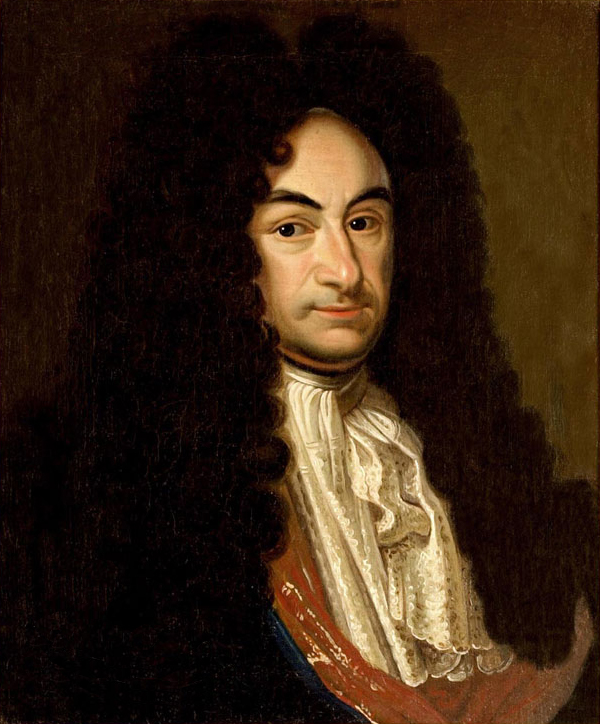
\includegraphics[width=0.7\linewidth]{Figure/L/Leibniz_Hannover}
\end{figure}
